\documentclass[a4paper,12pt]{article}

\usepackage{preamble}


\begin{document}

\begin{figure}[!ht]
\centering
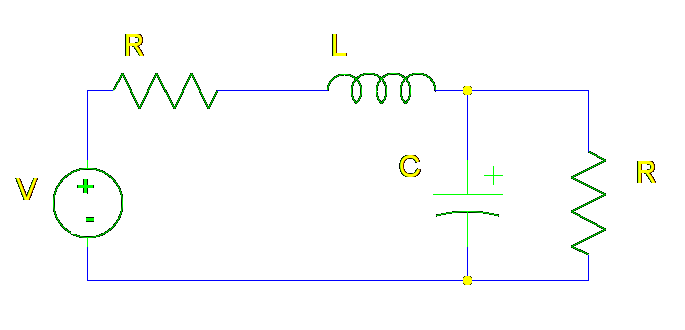
\includegraphics[width=8cm]{image/circuit.png}
\end{figure}

 A equação deste circuito 

 \[H(s) = \frac{\frac{R_2}{sCR_2+1}}{sL+R_1+\frac{R_2}{sCR_2+1}} = \frac{R_2}{(sL+R_1)(sCR_2+1)+R_2}
= \frac{\frac{1}{LC}}{s^2 + s\left(\frac{R_1}{L}+\frac{1}{R_2C}\right) +
\frac{1}{LC}+\frac{1}{LC}\frac{R_1}{R_2}},\]
 logo os pólos de $H$ são
 \[H(s) =\frac{ -\left(\frac{R_1}{L}+\frac{1}{R_2C}\right) \pm
\sqrt{\left(\frac{R_1}{L}+\frac{1}{R_2C}\right)^2 - 4\frac{1}{LC}\left(1+\frac{R_1}{R_2}\right)}}{2}\]








\end{document}
